\documentclass[10pt,a4paper]{article}

\usepackage[top=1cm,bottom=2cm]{geometry}
\usepackage{graphicx}
\usepackage[backend=bibtex]{biblatex}
\usepackage{hyperref}
\usepackage{xcolor}
\usepackage{listings}
\bibliography{report.bib}
\author{Christoffer Jansson \and Alan Khudur \and Dmitrij Lioubartsev \and Michal Staniaszek \and Yavor Trasiev}
\title{DD2425 Robotics and Autonomous Systems Final Report}

\begin{document}
\maketitle
\begin{abstract}
  In this report we describe our hardware and software solutions for the house
  service robot task set in the DD2425 Robotics and Autonomous Systems course.
  The task required the construction of a robot from a limited set of materials,
  and the implementation of a software system using the Robot Operating System
  (ROS)\cite{rosorg} framework. We implemented a control system for motion in
  the maze, including wall following, a vision system to make use of the
  Primesense RGB-D camera, and additional systems for mapping.
\end{abstract}
\section{Task Specification}
The website for the course specifies the task as follows:
\begin{quote}
  \emph{Your robot is the new service robot is someone's house. The new owner has just
  turned on the robot and given it a few minutes to have a look around in the
  new environment. Your robot should take this chance to learn as much as
  possible about the environment so that it can be as good as possible in future
  tasks. It should learn to find its way and it should detect and remember where
  certain objects are.}
\end{quote}
This specification is a description of a real world task that might be performed
by a robot. Since we had only two months to implement the system, the actual
task that had to be performed was somewhat simplified. The ``house'' was
replaced by a maze made of straight pieces of wood, with all of the walls having
either a horizontal or vertical orientation --- there are no diagonal walls. The
robot should detect and remember the location of are various brightly coloured
shapes, seen in Figure~\ref{fig:shapes}.

The task can be broken into two phases, each of which has a distinct purpose. In
the first phase, the robot must explore the environment and learn where objects
are. In the second phase, which is not described explicitly in the
specification, the robot should return to the previously discovered object
locations and ``fetch'' the objects.

Although these tasks would be trivial for any human, for a robot to do them
autonomously is a very demanding task, even in a restricted environment such as
the one we will be operating in. To complete the first phase, we must be able to
move the robot, which requires the implementation of controllers which allow the
robot to move based on demands on angular and linear velocity. A wall following
system is also required, to use the structure of the environment to explore it.
This requires the use of sensors to detect walls to the side and in front of the
robot to prevent collisions, and detect when it is possible for the robot to
turn. A vision system which can detect objects and correctly identify them is
also needed. A map must also be constructed and stored so that the position of
objects can be remembered for use in the second phase. During the second phase,
some sort of path planning is required to move efficiently between the different
objects. The ability to localise within the created map is also necessary in
order for the robot to know the position of objects and walls relative to its
own location. In addition, a way of navigating between specific locations in the
map is required.

To complete the full task, we had to design and build a robot, and write
software for all of these subsystems. The subsequent sections describe our
approach to each problem and how we solved it, including some of the ideas that
we did not use, and the reasons for that, as well as some analysis of the
performance of each of the subsystems.

\begin{figure}
  \centering
  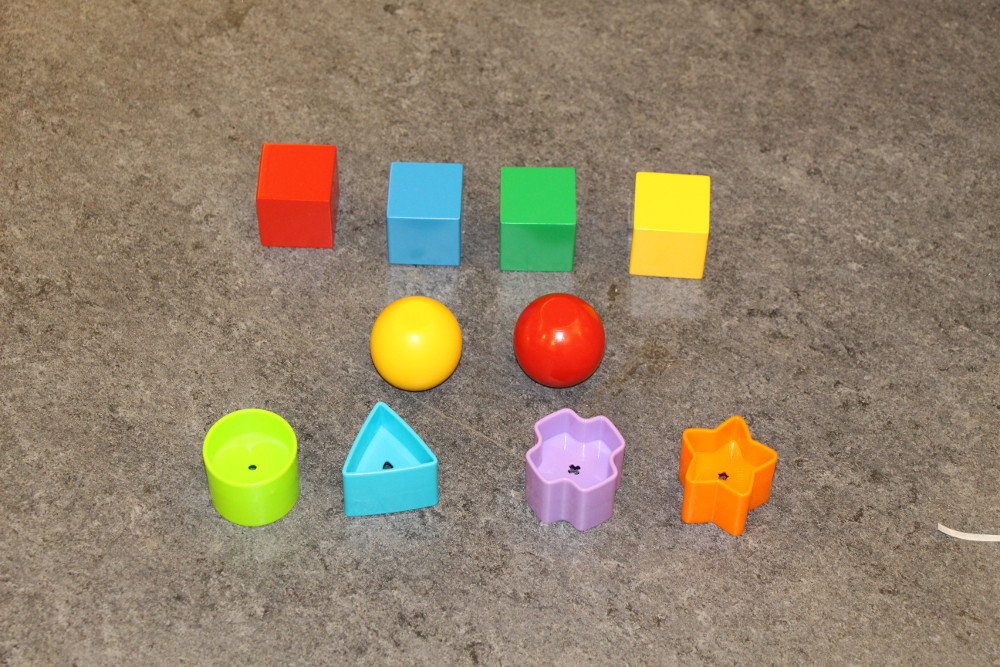
\includegraphics[width=\linewidth]{images/objects.jpg}
  \caption{Objects to be detected within the maze.}
  \label{fig:shapes}
\end{figure}
\section{Hardware}
\begin{figure}
  \centering
  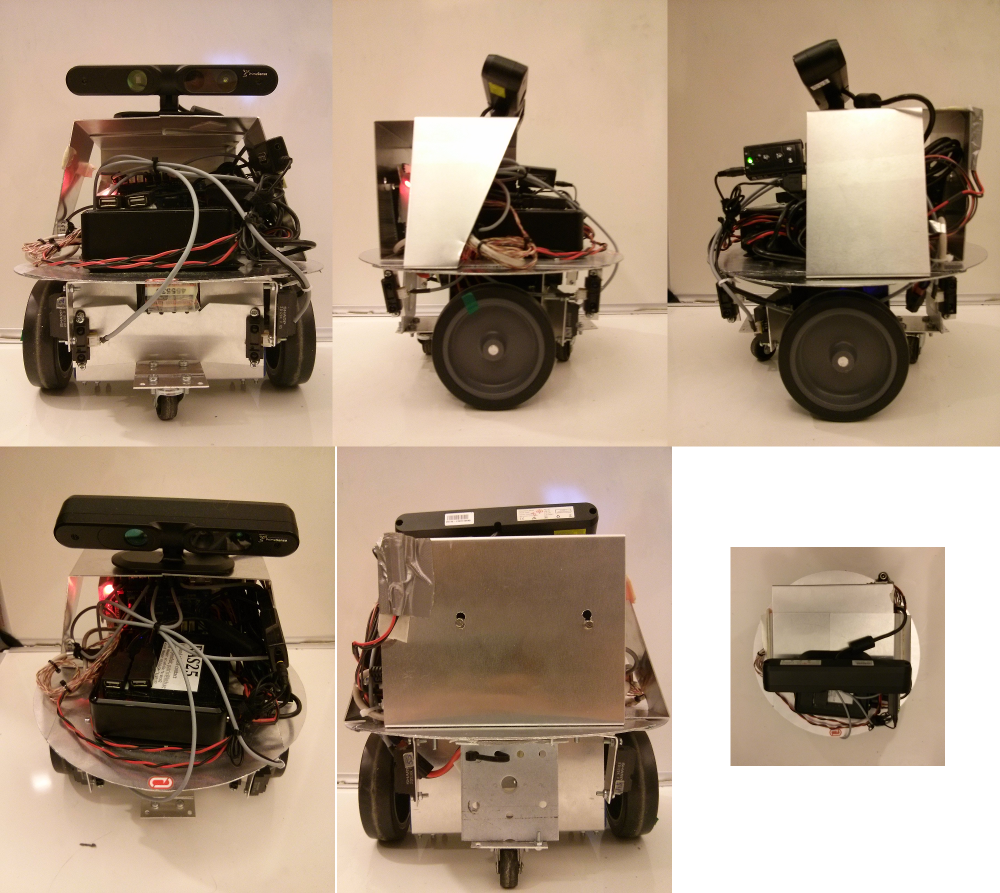
\includegraphics[width=\linewidth]{images/robo_views.png}
  \caption{Views of the robot from different angles.}
  \label{fig:roboview}
\end{figure}
\section{Controllers}
\section{Wall Following and Exploration}
\begin{figure}
  \centering
  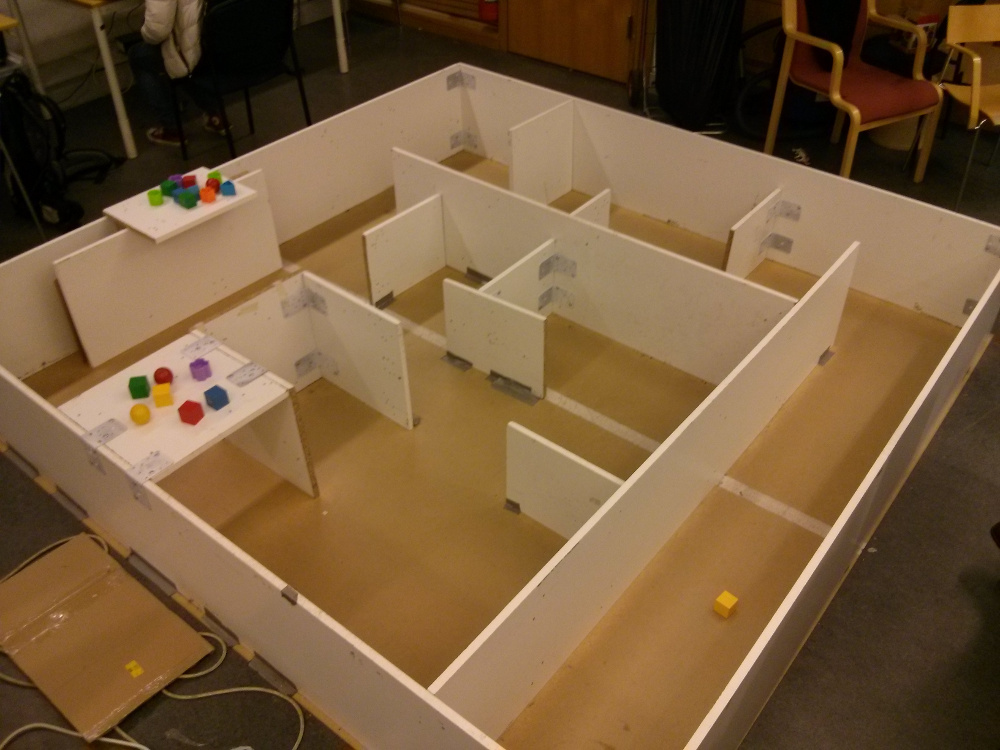
\includegraphics[width=\linewidth]{images/maze.jpg}
  \caption{The maze}
  \label{fig:maze}
\end{figure}
\section{Vision}
\section{Mapping}
In order to perform the task required in the second phase more efficiently, it
must be possible to 
\section{Localisation and Navigation}
\section{Work Environment}
\subsection{Version Control}
For source control, we used \texttt{git}, with repositories on GitHub. Each of
us had a separate account on GitHub, but we all committed to the same set of
repositories which were created in an Organisation on the site. We had separate
repositories for each major subsystem (mapping, controllers, vision, etc.).
Everyone committed to the same repositories, without using forks. While using
pull requests can have some benefits in terms of allowing team members to look
at what has been changed in a specific pull request and decide if changes are
required, in practice this sort of review process could only be done with a very
focused team that already have quite a lot of experience with \texttt{git}. It
would also be time consuming to have to do this, and time is already tight
enough as it is in the course. We tried to use a version of the branching model
described in \cite{nviebranch}. The idea is to use a branch \texttt{develop} in
each repository to develop code, branching off of that to develop new features,
in order not to force other members to pull code that is in the process of being
developed. The \texttt{master} branch is pushed to whenever a milestone
(release) is reached. While this may be a good branching model, in practice it
is perhaps not so useful if there is only one person working in a single
repository, as we often had. The good thing about it is that merging
\texttt{develop} into \texttt{master} only when a milestone is reached means
that the milestone code is easy to find, and it is possible to make sure that
only working code is merged.

There are some advantages to a multi-repository setup --- it is possible to work
on one repository completely independent of the others, which minimises the
number of merge commits and other issues that can be caused by having everything
in a single repository. The disadvantage of this is that all repositories have
to be pulled independently of each other, and if one forgets to do this it can
cause problems due to not having up to date code. The advantages of this setup
probably outweigh the disadvantages, however, because a single repository setup
would require more use of branches, which have issues of their own.

\subsection{System Setup}
At the beginning of the project we decided to make separate users on the NUC,
each with a separate \texttt{catkin} workspace. This worked well for us, as we
were able to work on different versions of code without affecting other members'
work. This came with the additional benefit that each member could launch their
own part of the code for a specific task independently. It did come with the
problem that each member had to pull updates to repositories, rather than having
a single repository which was up to date all the time. Each user belonged to the
same \texttt{robo} group, which allowed everyone to access each others' files. A
very useful script was one that allowed for execution of catkin make from any
directory, which saved having to switch between terminal windows or directories.
The system setup took some time, but the small amount of time spent at
the start was outweighed by the benefits.

\subsection{ROS Specifics}
We tried to keep to a specific structure for all nodes for consistency. Each
node created is an object (although there are no duplicated nodes). This keeps
the parameters of the node in its own scope, preventing possible issues with
clashes. Each node loads parameters and sets up subscribers in its constructor.
After all parameters are loaded, the node calls a function which executes the
main loop of the node. This structure makes it easy to see exactly what the node
is using by just looking at the constructor. In addition to this, we set up
parameter files for nodes which could use different parameter settings. Since
modifying extra parameters does not require recompilation, this saves time when
looking for the best parameter settings. A global parameter file was used to
store information about sensor positions and robot measurements. We make
extensive use of launch files as a result of this setup. Each launch file loads
the parameters that it requires. As such, it is possible to create a single
launch file at the top level which runs multiple nodes. Another parameter file
is used to define all topics that exist on the system. This means that one
change can change the name of the topic in all nodes which make use of it. This
means some additional parameter reading in nodes, but it lowers the likelihood
of bugs where nodes are not subscribing or publishing to the correct topics.

We implemented a utility library which was a wrapper around the parameter server
which would load a parameter into a given variable, depending on the type of the
variable. If the parameter was not present in the parameter server, an error
would be thrown with information about the missing parameter. This helped to
make parameter reading quicker and less prone to errors.

\section{Conclusion}

\nocite{*}
\printbibliography


\end{document}